\chapter{المخططات الثنائية صلب--سائل}\label{ch:b2:solid-liquid-diagrams}

ينصهر القصدير عند \qty{232}{\degreeCelsius} والرصاص عند \qty{327}{\degreeCelsius}،
ومع ذلك فإن لحام الكهربائيين القديم، وهو خليط منهما، ينصهر عند
\qty{182}{\degreeCelsius}، أي تحت درجتي انصهارهما. والملح المنثور على الطريق يذيب الجليد، لكن
حتى نحو \qty{-21}{\degreeCelsius} فقط؛ وفي ليلة أبرد لا يفعل شيئًا.
أما النحاس والنيكل فيمتزجان بأي نسبة حتى في الحالة
الصلبة، وتنصهر سبائكهما على مجال من درجات الحرارة بين درجتي انصهار
الفلزين. وتبيّن مخططات هذا الفصل، لكل زوج، أي الأجسام الصلبة
تتبلور من سائل يبرد، وعند أي درجات حرارة وبأي
كميات --- وهي المعرفة التي وراء كل صب، وكل وصلة لحام وكل
سبيكة منخفضة الانصهار.

\begin{recall}
\Cref{ch:b2:chemical-potential}: \omterm{def:b2:chemical-potential:chemical-potential}{الجهد الكيميائي} لمكوّن في \omterm{def:b2:chemical-potential:ideal-mixture}{خليط
مثالي}، وانخفاض درجة التجمد. \Cref{ch:b2:equilibrium-shifts}: \omterm{def:b2:equilibrium-shifts:variance}{التغايرية}.
\Cref{ch:b2:liquid-vapour-diagrams}: المخططات الثنائية، وخطوط الربط \omterm{thm:b2:liquid-vapour-diagrams:lever}{وقاعدة
الرافعة}. ومجلد السنة الأولى: الرابطة الفلزية، والسبائك الاستبدالية
والبينية، وأنماط البلورات.
\end{recall}

\begin{omfigure}
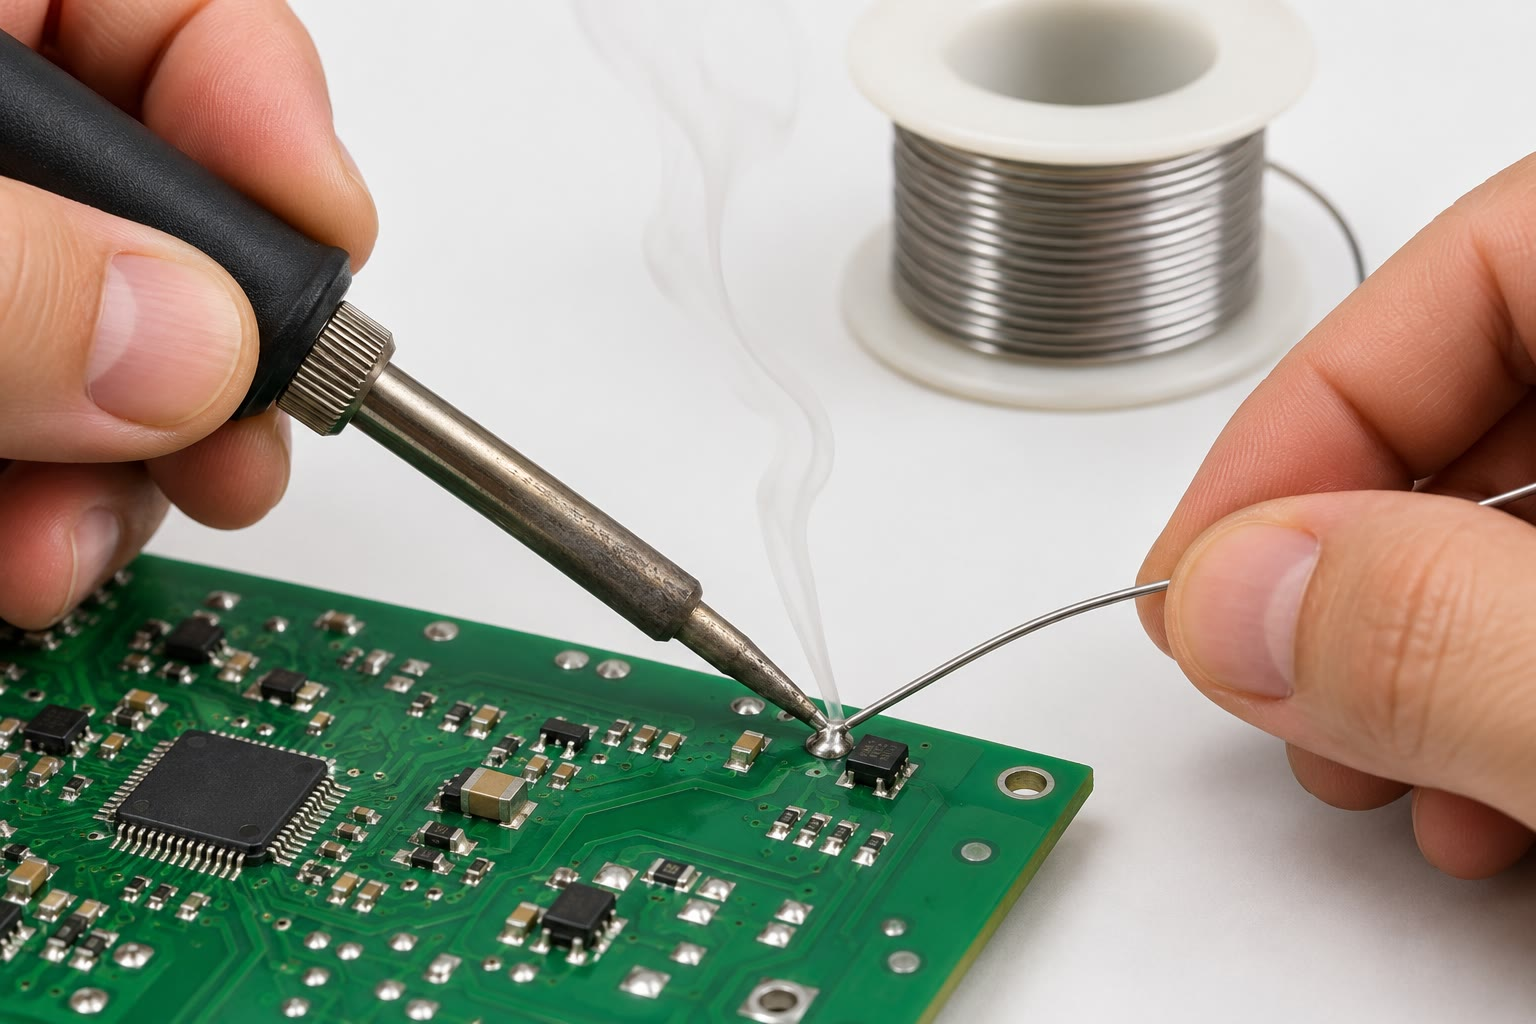
\includegraphics[width=0.6\linewidth]{images/book3/ai/b2-08-soldering.jpg}

{\small لحام مكوّن على لوحة دارة: يذوب سلك اللحام عند
تماسه بالكاوية الساخنة وتتجمد الوصلة في أقل من ثانية حين تُرفع
الكاوية --- لأن السبيكة تنصهر عند درجة حرارة واحدة منخفضة.}
\end{omfigure}

\section{التحليل الحراري}

\begin{definition}[التحليل الحراري]\label{def:b2:solid-liquid-diagrams:cooling-curve}
\emph{التحليل الحراري}\index{تحليل حراري} يحدد درجات حرارة
تغيرات الحالة لعيّنة انطلاقًا من درجة حرارتها المسجَّلة وهي
تُسخَّن أو تُبرَّد بمعدل ثابت. وتسجيل درجة الحرارة بدلالة الزمن
خلال تبريد بطيء هو \emph{منحنى التبريد}\index{منحنى التبريد}.
\end{definition}

بعيدًا عن أي تغيّر للحالة، تبرد العيّنة بانتظام. وحين يبدأ جسم صلب
بالتبلور، تبطئ حرارة التبلور التبريد: فيُظهر المنحنى
انكسارًا في الميل، أو يتوقف عند درجة حرارة ثابتة مدةً --- أي
\textit{استواءً} --- إذا جرى التجمد عند درجة حرارة ثابتة.

\begin{proposition}[الاستواءات]\label{prop:b2:solid-liquid-diagrams:plateaus}
عند ضغط ثابت، تتجمد المادة النقية عند درجة حرارة ثابتة، وكذلك
السائل الثنائي الذي يتبلور منه جسمان صلبان معًا. أما السائل الثنائي
الذي يتبلور منه جسم صلب واحد فيتجمد على مجال من درجات الحرارة.
\end{proposition}

\begin{proof}
عند ضغط مثبَّت تكون \omterm{def:b2:equilibrium-shifts:variance}{التغايرية} $v = n - r + 1 - \varphi$. مادة
نقية، سائل + جسم صلب: $v = 1 + 1 - 2 = 0$. نظام ثنائي، سائل + جسمان صلبان:
$v = 2 + 1 - 3 = 0$. نظام ثنائي، سائل + جسم صلب واحد: $v = 2 + 1 - 2 = 1$: فتتغير
درجة الحرارة مع تغيّر تركيب السائل. \omterm{def:b2:equilibrium-shifts:variance}{والتغايرية} 0 تعني أن درجة
الحرارة لا يمكن أن تتغير ما دامت الأطوار كلها موجودة: فالحرارة المنزوعة
يوفرها التجمد، حتى يختفي طور.
\end{proof}

\begin{omfigure}
\begin{tikzpicture}[font=\small, x=0.55cm, y=0.05cm]
  \foreach \dx/\name in {0/فلز نقي, 9/{خليط، يظهر جسم صلب أولًا}, 18/خليط أوتكتيكي} {
    \draw[->] (\dx,0) -- (\dx+7.5,0) node[below left, font=\scriptsize] {$t$};
    \draw[->] (\dx,0) -- (\dx,62) node[above, font=\scriptsize] {$T$};
    \node[font=\scriptsize] at (\dx+3.8,-8) {\name};
  }
  % pure: cool, plateau at 40, cool
  \draw[omDef, thick] (0,58) .. controls (1,48) and (1.6,42) .. (2,40) -- (4.5,40) .. controls (5.2,32) and (6,24) .. (7,20);
  \node[font=\scriptsize, anchor=south] at (3.25,40.5) {استواء};
  % mixture: cool, break at 48, slow fall, plateau at 30, cool
  \draw[omDef, thick] (9,58) .. controls (9.6,53) and (9.9,50) .. (10.2,48)
     .. controls (11,42) and (11.6,35) .. (12.3,30) -- (14.2,30) .. controls (14.9,23) and (15.6,17) .. (16.5,14);
  \node[font=\scriptsize, anchor=west] at (10.4,49.5) {انكسار};
  \node[font=\scriptsize, anchor=south] at (13.25,30.5) {أوتكتيك};
  % eutectic: plateau at 30
  \draw[omDef, thick] (18,58) .. controls (19,46) and (19.8,36) .. (20.5,30) -- (24,30) .. controls (24.7,23) and (25.4,17) .. (26.2,14);
  \node[font=\scriptsize, anchor=south] at (22.25,30.5) {استواء};
\end{tikzpicture}

{\small \omterm{def:b2:solid-liquid-diagrams:cooling-curve}{منحنيات تبريد}، رسم تخطيطي. يتجمد الفلز النقي على استواء. ويُظهر
الخليط انكسارًا في الميل حين يظهر أول جسم صلب، ثم التبريد
البطيء لسائل يتجمد على مجال من درجات الحرارة، ثم
استواء الأوتكتيك. أما السائل ذو التركيب الأوتكتيكي فيتجمد على
استواء واحد، كالمادة النقية.}
\end{omfigure}

\begin{method}[بناء مخطط من منحنيات التبريد]\label{met:b2:solid-liquid-diagrams:diagram-from-curves}
\begin{enumerate}
  \item سجّل \omterm{def:b2:solid-liquid-diagrams:cooling-curve}{منحنيات التبريد} لسلسلة من التراكيب، والمكوّنات النقية
        منها.
  \item على منحنى بياني (التركيب، درجة الحرارة)، ضع لكل تركيب
        درجة حرارة الانكسار الأول (بداية التبلور) ودرجة حرارة
        كل استواء.
  \item صِل نقاط بداية التبلور: فهذا \omterm{def:b2:solid-liquid-diagrams:liquidus}{خط السيولة}. وصِل
        نهايات التجمد: \omterm{def:b2:solid-liquid-diagrams:liquidus}{خط الصلابة}. والاستواء الموجود عند درجة الحرارة
        نفسها لتراكيب كثيرة خط لا متغير (أوتكتيك).
  \item طول الاستواء الأوتكتيكي، الأكبر عند التركيب
        الأوتكتيكي، يحدد موقع هذا التركيب.
\end{enumerate}
\end{method}

\section{الامتزاج التام في الحالة الصلبة}

\begin{definition}[المحلول الصلب]\label{def:b2:solid-liquid-diagrams:solid-solution}
\emph{المحلول الصلب}\index{محلول صلب} طور بلوري واحد متغير
التركيب، تحل فيه ذرات أحد المكوّنين محل ذرات
الآخر في مواقع الشبكة نفسها (استبدالي) أو تشغل فيه فجوات
تلك الشبكة (بيني).
\end{definition}

للنحاس والنيكل البنية المكعبة الممركزة الأوجه نفسها وذرات أنصاف
أقطارها متقاربة: فيكوّنان \omterm{def:b2:solid-liquid-diagrams:solid-solution}{محلولًا صلبًا} استبداليًا عند كل تركيب.

\begin{definition}[خط السيولة وخط الصلابة]\label{def:b2:solid-liquid-diagrams:liquidus}
على مخطط صلب--سائل، \emph{خط السيولة}\index{خط السيولة} هو المنحنى
الذي يكون كل شيء فوقه سائلًا؛ ويعطي تركيب السائل في
توازن مع جسم صلب. و\emph{خط الصلابة}\index{خط الصلابة} هو المنحنى الذي يكون
كل شيء تحته صلبًا؛ وحيث يكون الجسم الصلب محلولًا، يعطي
تركيب الجسم الصلب في توازن مع السائل.
\end{definition}

\begin{proposition}[العدسة]\label{prop:b2:solid-liquid-diagrams:lens}
إذا كوّن المكوّنان محاليل مثالية في السائل وفي الجسم الصلب،
وصل خطا السيولة والصلابة نقطتي الانصهار وأحاطا بمنطقة ذات
طورين على شكل عدسة؛ وعند كل درجة حرارة يرتبط الكسر المولي $x_i$
لكل مكوّن في السائل وفي الجسم الصلب بالعلاقة
\[
  \frac{x_i^{\ell}}{x_i^{s}} = \exp\left[-\frac{\Delta_{\text{انصهار}}H_i}{R}\left(\frac1T - \frac1{T_i^*}\right)\right] .
\]
\end{proposition}

\begin{proof}
للمكوّن $i$ \omterm{def:b2:chemical-potential:chemical-potential}{الجهد الكيميائي} نفسه في الطورين، $\mu_i^{*,s} +
RT\ln x_i^s = \mu_i^{*,\ell} + RT\ln x_i^\ell$، ومنه $RT\ln(x_i^\ell/x_i^s) =
-(\mu_i^{*,\ell} - \mu_i^{*,s}) = -\Delta_{\text{انصهار}}G_i(T)$، ومع
$\Delta_{\text{انصهار}}H_i$ ثابت، $\Delta_{\text{انصهار}}G_i = \Delta_{\text{انصهار}}H_i(1 - T/T_i^*)$.
ومع $x_1 + x_2 = 1$ في كل طور، تحدد العلاقتان التركيبين
عند كل $T$ (وقد حُلّتا عدديًا من أجل الشكل)؛ أما كون المنحنيين
الناتجين يكوّنان عدسة فنقبله.
\end{proof}

\begin{omfigure}
\begin{tikzpicture}
\begin{axis}[omphase, width=0.62\linewidth, height=7cm, ymin=1050, ymax=1480,
  xlabel={\shortstack{\foreignlanguage{arabic}{$x$ (النيكل)}}}, ylabel={\babelsublr{$T$ (\unit{\degreeCelsius})}}]
\addplot[omliquidus] table[x=xl, y=T] {figdata/out/bachelor-2-solid-liquid-a.dat};
\addplot[omsolidus] table[x=xs, y=T] {figdata/out/bachelor-2-solid-liquid-a.dat};
\draw[tieline] (axis cs:0.541,1300) -- (axis cs:0.609,1300);
\fill (axis cs:0.58,1300) circle (1.3pt);
\node[font=\scriptsize] at (axis cs:0.25,1400) {سائل};
\node[font=\scriptsize] at (axis cs:0.8,1150) {محلول صلب};
\node[font=\scriptsize, anchor=east] at (axis cs:0.5,1330) {خط السيولة};
\node[font=\scriptsize, anchor=west] at (axis cs:0.66,1290) {خط الصلابة};
\node[font=\scriptsize, anchor=west] at (axis cs:0.03,1080) {\qty{1085}{\degreeCelsius}};
\draw[black!50] (axis cs:0.005,1084) -- (axis cs:0.03,1080);
\node[font=\scriptsize, anchor=south east] at (axis cs:1.0,1456) {\qty{1455}{\degreeCelsius}};
\end{axis}
\end{tikzpicture}

{\small النحاس--النيكل، محسوبًا لمحلولين صلب وسائل مثاليين انطلاقًا من
درجتي انصهار الفلزين وأنتالبيي انصهارهما. وعند
\qty{1300}{\degreeCelsius} تنقسم سبيكة تركيبها 0.58 إلى سائل
تركيبه 0.541 وجسم صلب تركيبه 0.609 (خط الربط المتقطع).}
% ledger: tfus:Cu, dfus:Cu, tfus:Ni, dfus:Ni
\end{omfigure}

\begin{method}[قراءة مخطط صلب--سائل]\label{met:b2:solid-liquid-diagrams:read-solid-liquid}
\begin{enumerate}
  \item تتبّع الخط العمودي للتركيب الإجمالي نزولًا انطلاقًا من
        السائل.
  \item على \omterm{def:b2:solid-liquid-diagrams:liquidus}{خط السيولة} يظهر أول جسم صلب؛ ويُقرأ تركيبه على
        الطرف الآخر من خط الربط (\omterm{def:b2:solid-liquid-diagrams:liquidus}{خط الصلابة}، أو مكوّن نقي).
  \item في المنطقة ذات الطورين، اقرأ التركيبين عند طرفي خط
        الربط والنسبتين \omterm{thm:b2:liquid-vapour-diagrams:lever}{بقاعدة الرافعة}، بالمولات مع الكسور
        المولية، وبالكتلة مع الكسور الكتلية.
  \item على خط أفقي لا متغير، تتوقف درجة الحرارة حتى يختفي
        أحد الأطوار؛ وتحته، اقرأ الزوج الجديد من الأطوار.
\end{enumerate}
\end{method}

\begin{example}[سبيكة عند \qty{1300}{\degreeCelsius}]\label{ex:b2:solid-liquid-diagrams:lever}
للسبيكة التي كسرها المولي من النيكل 0.58 عند \qty{1300}{\degreeCelsius}، يكون
كسر الذرات الموجودة في الجسم الصلب $(0.58 - 0.541)/(0.609 - 0.541) = 0.57$.
وأول جسم صلب يظهر، قرب \qty{1315}{\degreeCelsius}، أغنى بالنيكل
من السبيكة، وآخر سائل أفقر.
\end{example}

يصف المخطط التوازن، وهو بطيء في الحالة الصلبة: فالبلورات الأولى،
الغنية بالنيكل، تغطيها طبقات تزداد فقرًا به كلما
تغير السائل، ولا يتسع الوقت للانتشار في الجسم الصلب كي يسويها. فالمصبوب
المبرَّد بسرعة يتكوّن من بلورات \textit{متدرجة التركيب}، تتغير من المركز إلى
الحافة؛ والتسخين الطويل تحت \omterm{def:b2:solid-liquid-diagrams:liquidus}{خط الصلابة} يجعلها متجانسة.

\section{انعدام الامتزاج في الحالة الصلبة: الأوتكتيك}

حين لا يمتزج الجسمان الصلبان إطلاقًا، يتبلور كل مكوّن نقيًا، ويكون
\omterm{def:b2:solid-liquid-diagrams:liquidus}{لخط السيولة} فرعان، فرع لكل جسم صلب.

\begin{theorem}[شرودر--فان لار]\label{thm:b2:solid-liquid-diagrams:schroder}
إذا تبلور مكوّن A نقيًا من خليط سائل مثالي، فإن \omterm{def:b2:solid-liquid-diagrams:liquidus}{خط السيولة}
الذي يظهر عليه الجسم الصلب A تعطيه العلاقة
\[
  \ln x_A = -\frac{\Delta_{\text{انصهار}}H_A}{R}\Big(\frac1T - \frac1{T_A^*}\Big),
\]
حيث $x_A$ الكسر المولي للمكوّن A في السائل، و$T_A^*$ 
و$\Delta_{\text{انصهار}}H_A$ درجة انصهار A النقي وأنتالبي انصهاره
(المأخوذ ثابتًا).
\end{theorem}

\begin{proof}
عند التوازن، يساوي \omterm{def:b2:chemical-potential:chemical-potential}{الجهد الكيميائي} للجسم الصلب A النقي جهد A في
السائل: $\mu_A^{*,s}(T) = \mu_A^{*,\ell}(T) + RT\ln x_A$. ومنه $R\ln x_A =
-\Delta_{\text{انصهار}}G_A(T)/T$. وحسب جيبس--هلمهولتز، $d(\Delta_{\text{انصهار}}G_A/T)/
dT = -\Delta_{\text{انصهار}}H_A/T^2$؛ وبالمكاملة من $T_A^*$، حيث
$\Delta_{\text{انصهار}}G_A = 0$، إلى $T$ نحصل على $\Delta_{\text{انصهار}}G_A/T =
\Delta_{\text{انصهار}}H_A(1/T - 1/T_A^*)$.
\end{proof}

من أجل محلول مخفف، $\ln x_A = \ln(1 - x_B) \approx -x_B$ و$1/T -
1/T_A^* \approx -\Delta T/T_A^{*2}$: $\Delta T = RT_A^{*2}x_B/\Delta_{\text{انصهار}}H_A$،
وهو القانون الكريوسكوبي في \cref{ch:b2:chemical-potential}. ومن أجل البنزين ($T^* =
\qty{278.64}{K}$، $\Delta_{\text{انصهار}}H = \qty{9.87}{kJ/mol}$، $M =
\qty{78.11}{g/mol}$)، يخرج \omterm{def:b2:chemical-potential:colligative}{الثابت الكريوسكوبي} $RT^{*2}M/\Delta_{\text{انصهار}}H$
مساويًا \qty{5.11}{K.kg/mol}.
% ledger: tfus:benzene, dfus:benzene

\begin{definition}[الأوتكتيك]\label{def:b2:solid-liquid-diagrams:eutectic}
\emph{النقطة الأوتكتيكية}\index{نقطة أوتكتيكية} لنظام ثنائي هي
النقطة التي يكون فيها السائل في توازن مع جسمين صلبين معًا؛ وهي
أدنى درجة حرارة يوجد عندها سائل في ذلك الجزء من المخطط. والسائل
ذو التركيب الأوتكتيكي، والخليط الدقيق المتداخل من الجسمين
الصلبين الذي يتجمد إليه، يُسمّيان \emph{خليطًا
أوتكتيكيًا}\index{خليط أوتكتيكي}.
\end{definition}

\begin{corollary}[الأوتكتيك هو ملتقى فرعي خط السيولة]\label{cor:b2:solid-liquid-diagrams:eutectic}
من أجل مكوّنين غير قابلين للامتزاج في الحالة الصلبة ومثاليين في السائل، تكون
درجة الحرارة الأوتكتيكية $T_E$ والتركيب الأوتكتيكي حل المعادلة
$x_A(T_E) + x_B(T_E) = 1$، حيث يعطي كل $x$ معادلةُ شرودر--فان لار
لجسمه الصلب.
\end{corollary}

\begin{proof}
عند الأوتكتيك يكون السائل مشبعًا بالجسمين الصلبين: فيقع على
الفرعين معًا، بالتركيب نفسه مقروءًا بدلالة A وبدلالة B.
\end{proof}

\begin{omfigure}
\begin{tikzpicture}
\begin{axis}[omphase, width=0.62\linewidth, height=6.5cm, ymin=-25, ymax=85,
  xlabel={\shortstack{\foreignlanguage{arabic}{$x$ (النفثالين)}}}, ylabel={\babelsublr{$T$ (\unit{\degreeCelsius})}}]
\addplot[omliquidus] table[x=x, y=T] {figdata/out/bachelor-2-solid-liquid-b-benzene.dat};
\addplot[omliquidus] table[x=x, y=T] {figdata/out/bachelor-2-solid-liquid-b-naphthalene.dat};
\draw[thick] (axis cs:0,-3.55) -- (axis cs:1,-3.55);
\fill (axis cs:0.133,-3.55) circle (1.5pt);
\node[font=\scriptsize, anchor=north] at (axis cs:0.133,-4.5) {E};
\node[font=\scriptsize] at (axis cs:0.45,72) {سائل};
\node[font=\scriptsize, align=center] at (axis cs:0.65,22) {سائل + نفثالين\\ صلب};
\node[font=\scriptsize, anchor=south west] at (axis cs:0.08,45) {سائل + بنزين صلب};
\draw[thin] (axis cs:0.12,45) -- (axis cs:0.06,0.8);
\node[font=\scriptsize] at (axis cs:0.55,-15) {بنزين صلب + نفثالين صلب};
\end{axis}
\end{tikzpicture}

{\small البنزين--النفثالين، محسوبًا بمعادلة شرودر--فان لار
لكل جسم صلب. يلتقي الفرعان عند الأوتكتيك E،
\qty{-3.5}{\degreeCelsius} و0.13 من النفثالين، وكل شيء تحته صلب.}
% ledger: tfus:benzene, dfus:benzene, tfus:naphthalene, dfus:naphthalene
\end{omfigure}

\begin{example}[تبريد خليط بنزين--نفثالين]\label{ex:b2:solid-liquid-diagrams:naphthalene}
يبرد سائل كسره المولي من النفثالين 0.5 حتى يبلغ فرع النفثالين
من \omterm{def:b2:solid-liquid-diagrams:liquidus}{خط السيولة}، قرب \qty{46}{\degreeCelsius}، حيث يبدأ النفثالين الصلب النقي
بالتبلور. فينزلق السائل، الذي يفقد النفثالين، على طول
الفرع؛ وعند \qty{-3.5}{\degreeCelsius} يبلغ الأوتكتيك، ويتجمد الباقي
عند درجة حرارة ثابتة إلى \omterm{def:b2:solid-liquid-diagrams:eutectic}{الخليط الأوتكتيكي}. وبقاعدة الرافعة،
فوق الأوتكتيك مباشرة، يمثل النفثالين الصلب $(0.5 - 0.133)/(1 - 0.133) =
42~\%$ من المولات، والسائل الأوتكتيكي 58~\%.
\end{example}

\begin{proposition}[طول الاستواء الأوتكتيكي]\label{prop:b2:solid-liquid-diagrams:plateau-length}
من أجل عيّنات متساوية الكتلة تُبرَّد بالمعدل نفسه لنزع الحرارة، تتناسب
مدة الاستواء الأوتكتيكي مع كمية السائل التي
تبلغ الأوتكتيك، فتكون عظمى عند التركيب الأوتكتيكي ومعدومة عند
المكوّنين النقيين.
\end{proposition}

\begin{proof}
على الاستواء تكون درجة الحرارة ثابتة: فالحرارة المنزوعة، $\Phi\,\Delta t$
بمعدل ثابت $\Phi$، هي الحرارة التي يحررها تجمد السائل
الأوتكتيكي، $m_E\,\Delta_{\text{انصهار}}h_E$. ومنه $\Delta t = m_E\,\Delta_{\text{انصهار}}h_E/
\Phi$، المتناسب مع الكتلة $m_E$ للسائل الأوتكتيكي، التي تعطيها \omterm{thm:b2:liquid-vapour-diagrams:lever}{قاعدة
الرافعة}.
\end{proof}

\section{الامتزاج الجزئي والمركبات المحدَّدة}

أغلب أزواج الفلزات ليست تامة الامتزاج ولا تامة عدم الامتزاج في الحالة
الصلبة: فكل منهما يذيب قليلًا من الآخر. فالرصاص يذيب حتى 19~\% من القصدير
كتلةً، والقصدير حتى 3.4~\% من الرصاص. فيحوي المخطط عندئذ \omterm{def:b2:solid-liquid-diagrams:solid-solution}{محلولين
صلبين}، (Pb) و(Sn)، وأوتكتيكًا بينهما؛ ولا يعود الخط الأوتكتيكي
يبلغ جانبي المخطط، بل يتوقف عند حدود \omterm{def:b2:solid-liquid-diagrams:solid-solution}{المحلولين
الصلبين}.

\begin{omfigure}
\begin{tikzpicture}[font=\small, x=0.075cm, y=0.022cm]
  \draw[->] (0,0) -- (106,0) node[right] {\shortstack{\foreignlanguage{arabic}{\babelsublr{\% Sn} (كتلةً)}}};
  \draw[->] (0,0) -- (0,360) node[above] {$T$ (\unit{\degreeCelsius})};
  \foreach \t in {100,200,300} \draw (0,\t) -- (-1.5,\t) node[left, font=\scriptsize] {\t};
  \foreach \w in {0,20,40,60,80,100} \draw (\w,0) -- (\w,-5) node[below, font=\scriptsize] {\w};
  % invariant points (NIST): Pb 327.5, Sn 231.9, eutectic 182.2 at 62.13; limits 18.91 and 96.59
  \draw[omliquidus] (0,327.5) .. controls (25,290) and (45,235) .. (62.13,182.2);
  \draw[omliquidus] (100,231.9) .. controls (85,215) and (72,200) .. (62.13,182.2);
  \draw[omsolidus] (0,327.5) .. controls (8,280) and (14,220) .. (18.91,182.2);
  \draw[omsolidus] (100,231.9) .. controls (98.5,215) and (97.5,200) .. (96.59,182.2);
  \draw[thick] (18.91,182.2) -- (96.59,182.2);
  \draw[omsolidus, densely dashed] (18.91,182.2) .. controls (12,120) and (6,60) .. (3,20);
  \draw[omsolidus, densely dashed] (96.59,182.2) .. controls (98.5,120) and (99.3,60) .. (99.6,20);
  \fill (62.13,182.2) circle (1.5pt);
  \fill (18.91,182.2) circle (1.2pt); \fill (96.59,182.2) circle (1.2pt);
  \node[anchor=south, font=\scriptsize] at (62.13,186) {E};
  \node[font=\scriptsize] at (55,300) {سائل};
  \node[font=\scriptsize] at (6,150) {(Pb)};
  \node[font=\scriptsize] at (103,140) {(Sn)};
  \node[font=\scriptsize] at (28,235) {L + (Pb)};
  \node[font=\scriptsize] at (84,192) {L + (Sn)};
  \node[font=\scriptsize] at (55,100) {(Pb) + (Sn)};
  % cooling path at 40 %
  \draw[->, omProp, thick] (40,340) -- (40,30);
  \node[font=\scriptsize, omProp, anchor=south] at (40,342) {40~\%};
  \node[font=\scriptsize, anchor=north east] at (16.6,179) {18.9};
  \node[font=\scriptsize, anchor=north] at (62.13,178) {62.1};
  \node[font=\scriptsize, anchor=north east] at (95.8,178) {96.6};
  \node[font=\scriptsize, anchor=west] at (101,182.2) {\qty{182.2}{\degreeCelsius}};
\end{tikzpicture}

{\small مخطط الرصاص--القصدير، مرسومًا عبر نقاطه اللامتغيرة: درجتا
انصهار الرصاص (\qty{327.5}{\degreeCelsius}) والقصدير (\qty{231.9}{\degreeCelsius})،
والأوتكتيك E عند \qty{182.2}{\degreeCelsius} و62.1~\% من القصدير، وحدّا \omterm{def:b2:solid-liquid-diagrams:solid-solution}{المحلولين
الصلبين} عند درجة الحرارة الأوتكتيكية (18.9~\% و96.6~\% من القصدير). أما المنحنيات
بين هذه النقاط، وحدود الذوبانية المتقطعة تحت الأوتكتيك،
فمرسومة رسمًا تخطيطيًا. السهم: تبريد لحام نسبته 40~\%.}
% ledger: eut:Pb-Sn.T, eut:Pb-Sn.wL, eut:Pb-Sn.wPb, eut:Pb-Sn.wSn, tfus:Pb, tfus:Sn
\end{omfigure}

يبدأ لحام نسبة القصدير فيه 40~\% بالتجمد على \omterm{def:b2:solid-liquid-diagrams:liquidus}{خط السيولة} بترسيب بلورات
من المحلول الغني بالرصاص (Pb)؛ ويغتني السائل بالقصدير حتى يبلغ،
عند \qty{182.2}{\degreeCelsius}، التركيب الأوتكتيكي فيتجمد إلى
خليط دقيق من صفائح (Pb) و(Sn)، حول البلورات الأولية.

\begin{omfigure}
\begin{tikzpicture}[font=\small]
  \begin{scope}
    \clip (0,0) circle (2.2);
    \fill[gray!20] (-2.3,-2.3) rectangle (2.3,2.3);
    \foreach \k in {-24,...,24} \draw[gray!65, line width=1.1pt] (-2.4+0.2*\k,-2.4) -- ++(55:6);
    \foreach \cx/\cy/\r/\a in {-0.9/0.8/0.55/10, 0.7/1.0/0.45/40, 0.2/-0.6/0.6/-20, -1.1/-0.9/0.4/70, 1.3/-0.3/0.35/5} {
      \fill[omDef!35, draw=omDef, rotate around={\a:(\cx,\cy)}] (\cx,\cy) ellipse ({\r} and {0.7*\r});
    }
  \end{scope}
  \draw[thick] (0,0) circle (2.2);
  \draw[<-, omProp, thick] (0.7,1.0) -- (3.0,1.6) node[right, text=black] {\foreignlanguage{arabic}{بلورة أولية من \babelsublr{(Pb)}}};
  \draw[<-, omProp, thick] (1.6,0.9) -- (3.0,0.5) node[right, text=black, align=left] {\foreignlanguage{arabic}{أوتكتيك: صفائح متناوبة}\\ \foreignlanguage{arabic}{من \babelsublr{(Pb)} و\babelsublr{(Sn)}}};
\end{tikzpicture}

{\small البنية المجهرية للحام فيه 40~\% من القصدير بعد تبريد بطيء، رسم تخطيطي:
بلورات أولية من (Pb)، تكوّنت بين \omterm{def:b2:solid-liquid-diagrams:liquidus}{خط السيولة} والأوتكتيك، في
أرضية أوتكتيكية مكوّنة من صفائح رقيقة متناوبة من \omterm{def:b2:solid-liquid-diagrams:solid-solution}{المحلولين
الصلبين}.}
\end{omfigure}

\begin{definition}[المركب المحدَّد]\label{def:b2:solid-liquid-diagrams:defined-compound}
\emph{المركب المحدَّد}\index{مركب محدد} جسم صلب ثابت
التركيب $\mathrm{A}_a\mathrm{B}_b$ يكوّنه المكوّنان. ويُظهر
\emph{انصهارًا متطابقًا}\index{انصهار متطابق} حين ينصهر إلى سائل له
تركيبه نفسه: فيكون \omterm{def:b2:solid-liquid-diagrams:liquidus}{لخط السيولة} عندئذ قيمة عظمى عند ذلك التركيب.
\end{definition}

المركب ذو \omterm{def:b2:solid-liquid-diagrams:defined-compound}{الانصهار المتطابق} يقسم المخطط قسمين: فكل نصف، A مع
$\mathrm{A}_a\mathrm{B}_b$ و$\mathrm{A}_a\mathrm{B}_b$ مع B، مخطط
مستقل، له أوتكتيكه الخاص. وتركيب القيمة العظمى، مقروءًا بالكسر
المولي، يعطي صيغة المركب.

\begin{omfigure}
\begin{tikzpicture}[font=\small, x=6cm, y=0.05cm]
  \draw[->] (0,0) -- (1.06,0) node[right] {$x_{\mathrm B}$};
  \draw[->] (0,0) -- (0,95) node[above] {$T$};
  \node[below, font=\scriptsize] at (0,0) {A}; \node[below, font=\scriptsize] at (1,0) {B};
  \node[below, font=\scriptsize] at (0.667,0) {$\tfrac23$};
  \draw[omliquidus] (0,70) .. controls (0.12,58) and (0.25,45) .. (0.35,35);
  \draw[omliquidus] (0.35,35) .. controls (0.45,62) and (0.58,79) .. (0.667,80);
  \draw[omliquidus] (0.667,80) .. controls (0.75,79) and (0.8,68) .. (0.85,50);
  \draw[omliquidus] (0.85,50) .. controls (0.9,56) and (0.95,62) .. (1,65);
  \draw[thick] (0,35) -- (0.667,35); \draw[thick] (0.667,50) -- (1,50);
  \draw[thick] (0.667,0) -- (0.667,80);
  \fill (0.35,35) circle[radius=1.5pt]; \fill (0.85,50) circle[radius=1.5pt];
  \fill (0.667,80) circle[radius=1.5pt];
  \node[anchor=north, font=\scriptsize] at (0.35,34) {E$_1$};
  \node[anchor=north, font=\scriptsize] at (0.85,49) {E$_2$};
  \node[anchor=south, font=\scriptsize] at (0.667,81) {\foreignlanguage{arabic}{انصهار $\mathrm{AB_2}$}};
  \node[font=\scriptsize] at (0.35,80) {سائل};
  \node[font=\scriptsize, align=center] at (0.33,15) {A +\\ $\mathrm{AB_2}$};
  \node[font=\scriptsize, align=center] at (0.84,25) {$\mathrm{AB_2}$\\ + B};
\end{tikzpicture}

{\small مخطط تخطيطي فيه مركب محدَّد $\mathrm{AB_2}$ (الخط
العمودي عند $x_{\mathrm B} = 2/3$) ينصهر \omterm{def:b2:solid-liquid-diagrams:defined-compound}{انصهارًا متطابقًا} عند القيمة العظمى \omterm{def:b2:solid-liquid-diagrams:liquidus}{لخط
السيولة}. فالمخطط مخططان أوتكتيكيان بسيطان متجاوران، لهما
الأوتكتيكان E$_1$ وE$_2$.}
\end{omfigure}

\section{تطبيقات}

\paragraph{أنواع اللحام والسبائك المنخفضة الانصهار.} يجب أن ينصهر اللحام تحت درجة انصهار القطع
التي يصلها وأن يتجمد بسرعة، دون مجال عجيني: فالتركيب الأوتكتيكي هو
الاختيار الطبيعي. وأوتكتيك القصدير--الرصاص ينصهر عند \qty{182.2}{\degreeCelsius}؛
ولأن الرصاص سام، تستعمل الإلكترونيات اليوم أنواع لحام خالية من الرصاص، منها
أوتكتيك البزموت--القصدير، الذي ينصهر عند \qty{138.8}{\degreeCelsius} ويحوي
57~\% من البزموت كتلةً.
% ledger: eut:Pb-Sn.T, eut:Bi-Sn.T, eut:Bi-Sn.wL

\paragraph{إزالة الجليد.} يكوّن الجليد والملح أوتكتيكًا: فأوتكتيك الجليد--ثنائي هيدرات
الملح يقع عند \qty{252}{K} (\qty{-21}{\degreeCelsius}) و23.3~\% من كلوريد
الصوديوم كتلةً. وفوق هذه الدرجة يكوّن الملح الملامس للجليد
محلولًا ملحيًا درجة تجمده أدنى من درجة حرارة الطريق، فيذوب الجليد؛
وتحتها لا يمكن أن يوجد أي سائل، فلا فائدة من الملح.
% ledger: eut:NaCl-water.T, eut:NaCl-water.w

\paragraph{التبلور.} يُقرأ مخطط ملح وماء كأي مخطط
آخر: فتبريد محلول ساخن مشبع يعبر منحنى الذوبانية (\omterm{def:b2:solid-liquid-diagrams:liquidus}{خط
السيولة} للملح)، فتترسب بلورات نقية من الملح بينما
تبقى الشوائب، المخففة أكثر من أن تبلغ خطوط سيولتها، في المحلول الأم.
وهذه هي التنقية بإعادة التبلور الواردة في مجلد السنة الأولى، مرئيةً على
مخطط.

\begin{omfigure}
\begin{tikzpicture}
\begin{axis}[omphase, width=0.62\linewidth, height=6cm, xmin=0, xmax=100,
  ymin=90, ymax=285, xlabel={\shortstack{\foreignlanguage{arabic}{\babelsublr{\% Bi} (كتلةً)}}}, ylabel={\babelsublr{$T$ (\unit{\degreeCelsius})}}]
\addplot[omliquidus] table[x=w, y=T] {figdata/out/bachelor-2-solid-liquid-d-Sn.dat};
\addplot[omliquidus] table[x=w, y=T] {figdata/out/bachelor-2-solid-liquid-d-Bi.dat};
\draw[densely dashed] (axis cs:0,119.5) -- (axis cs:100,119.5);
\fill[omThm] (axis cs:56.97,138.8) circle (2pt);
\node[font=\scriptsize, omThm, anchor=west] at (axis cs:64,129) {الأوتكتيك المقيَّم};
\draw[omThm, thin] (axis cs:64,129) -- (axis cs:57.8,137.6);
\node[font=\scriptsize, anchor=north] at (axis cs:52,118) {النموذج المثالي};
\node[font=\scriptsize] at (axis cs:50,250) {سائل};
\end{axis}
\end{tikzpicture}

{\small البزموت--القصدير: \omterm{def:b2:solid-liquid-diagrams:liquidus}{خط السيولة} المتنبأ به لجسمين صلبين نقيين وسائل
مثالي (شرودر--فان لار، بالأزرق) يلتقي فرعاه عند أوتكتيك قرب
\qty{120}{\degreeCelsius}؛ أما الأوتكتيك المقيَّم (النقطة الحمراء) فيقع عند
\qty{138.8}{\degreeCelsius} و57~\% من البزموت.}
% ledger: tfus:Sn, dfus:Sn, tfus:Bi, dfus:Bi, eut:Bi-Sn.T, eut:Bi-Sn.wL
\end{omfigure}

\section{تمارين}

\begin{exercise}[$\star$]\label{exo:b2:solid-liquid-diagrams:1}
على مخطط النحاس--النيكل، اذكر الأطوار الموجودة عند
\qty{1300}{\degreeCelsius} للكسور المولية من النيكل 0.40 و0.58 و0.70.
\end{exercise}

\begin{exercise}[$\star$]\label{exo:b2:solid-liquid-diagrams:2}
يُحفظ \qty{2.00}{mol} من سبيكة نحاس--نيكل كسرها المولي من النيكل 0.58
عند \qty{1300}{\degreeCelsius}. احسب كميتي الجسم الصلب والسائل وكمية
النيكل في كل منهما.
\end{exercise}

\begin{exercise}[$\star$]\label{exo:b2:solid-liquid-diagrams:3}
احسب \omterm{def:b2:equilibrium-shifts:variance}{التغايرية} عند ضغط ثابت (أ) لفلز نقي وهو يتجمد؛
(ب) لسبيكة نحاس--نيكل وهي تتجمد؛ (ج) لسائل رصاص--قصدير على
الخط الأوتكتيكي.
\end{exercise}

\begin{exercise}[$\star$]\label{exo:b2:solid-liquid-diagrams:4}
ارسم بخطوط تقريبية منحنى تبريد القصدير النقي من \qty{300}{\degreeCelsius} إلى
\qty{100}{\degreeCelsius} وفسّر لماذا تتوقف درجة الحرارة عند
\qty{232}{\degreeCelsius}.
\end{exercise}

\begin{exercise}[$\star\star$]\label{exo:b2:solid-liquid-diagrams:5}
مستعملًا معطيات الفصل (البنزين \qty{278.64}{K}، \qty{9.87}{kJ/mol}؛
والنفثالين \qty{353.2}{K}، \qty{19.1}{kJ/mol})، تحقق من أن الكسرين الموليين
لشرودر--فان لار عند \qty{269.6}{K} مجموعهما 1، وأعطِ
التركيب الأوتكتيكي.
\end{exercise}

\begin{exercise}[$\star\star$]\label{exo:b2:solid-liquid-diagrams:6}
صِف تبريد سبيكة رصاص--قصدير فيها 30~\% من القصدير كتلةً، من السائل
إلى درجة حرارة الغرفة، واحسب الكسر الكتلي للأوتكتيك الذي تحويه.
\end{exercise}

\begin{exercise}[$\star\star$]\label{exo:b2:solid-liquid-diagrams:7}
ما كتلة كلوريد الصوديوم لكل كيلوغرام من الماء في المحلول الملحي
الأوتكتيكي؟ ولماذا لا يفيد تمليح الطريق عند \qty{-25}{\degreeCelsius}؟
\end{exercise}

\begin{exercise}[$\star\star$]\label{exo:b2:solid-liquid-diagrams:8}
على المخطط التخطيطي الذي فيه المركب $\mathrm{AB_2}$، صِف
تبريد سائلين فيهما $x_{\mathrm B} = 0.5$ و$x_{\mathrm B} = 0.9$: أول
جسم صلب، والأوتكتيك المبلوغ، والأجسام الصلبة في النهاية.
\end{exercise}

\begin{exercise}[$\star\star$]\label{exo:b2:solid-liquid-diagrams:9}
في التنقية بالمنطقة المنصهرة، تُمرَّر منطقة منصهرة ببطء على طول قضيب. وقرب النيكل النقي،
تساوي نسبة الكسرين الموليين للنحاس في الجسم الصلب وفي السائل عند
التوازن نحو 0.78. فسّر لماذا ينتقل النحاس مع
المنطقة المنصهرة، ولماذا تلزم عدة تمريرات.
\end{exercise}

\begin{exercise}[$\star\star\star$]\label{exo:b2:solid-liquid-diagrams:10}
استنتج معادلة شرودر--فان لار، ثم بيّن أنها تؤول من أجل سائل مخفف
إلى $\Delta T = K_f\,b$، مع $K_f = RT^{*2}M_A/\Delta_{\text{انصهار}}H_A$
و$b$ مولالية المذاب؛ واحسب $K_f$ للبنزين.
\end{exercise}

\begin{exercise}[$\star\star\star$]\label{exo:b2:solid-liquid-diagrams:11}
لمخطط المغنيسيوم--الرصاص قيمة عظمى \omterm{def:b2:solid-liquid-diagrams:liquidus}{لخط السيولة} عند 19.0~\% من المغنيسيوم
كتلةً. أوجد صيغة المركب.
\end{exercise}

\begin{exercise}[$\star\star\star$]\label{exo:b2:solid-liquid-diagrams:12}
تُبرَّد كتل متساوية من سبائك رصاص--قصدير في الشروط نفسها. فتُظهر
السبيكة الأوتكتيكية استواءً مدته \qty{300}{s}؛ وتُظهر سبيكة مجهولة استواءً مدته
\qty{120}{s}. أوجد التركيبين الممكنين للسبيكة المجهولة، وبيّن كيف
تميّز بينهما.
\end{exercise}

\section{مسألة: اللحام}

\begin{problem}[{مسألة نهاية الأسبوع --- مخطط الرصاص--القصدير من نقاطه
اللامتغيرة، وتجمد لحام نسبته 40~\% بقاعدة الرافعة، ولحام خالٍ من الرصاص
من البزموت--القصدير يتنبأ به نموذج السائل المثالي، واختيار
لحام}]
\label{pb:b2:solid-liquid-diagrams:1}
المعطيات (NIST، التوازنات اللامتغيرة المحسوبة): أوتكتيك الرصاص--القصدير عند
\qty{182.2}{\degreeCelsius}، سائل فيه 62.13~\% من القصدير كتلةً، في توازن مع
(Pb) فيه 18.91~\% و(Sn) فيه 96.59~\% من القصدير؛ وأوتكتيك البزموت--القصدير عند
\qty{138.8}{\degreeCelsius}، سائل فيه 56.97~\% من البزموت. درجات الانصهار
وأنتالبيات الانصهار: الرصاص \qty{600.6}{K}، \qty{4.77}{kJ/mol}؛ القصدير
\qty{505.1}{K}، \qty{7.03}{kJ/mol}؛ البزموت \qty{544.6}{K}، \qty{11.30}{kJ/mol}.
الكتل المولية (\unit{g/mol}): Pb 207.2، Sn 118.71، Bi 208.98.
% ledger: eut:Pb-Sn.T, eut:Pb-Sn.wL, eut:Pb-Sn.wPb, eut:Pb-Sn.wSn, eut:Bi-Sn.T, eut:Bi-Sn.wL, tfus:Pb, dfus:Pb, tfus:Sn, dfus:Sn, tfus:Bi, dfus:Bi, aw:Pb, aw:Sn, aw:Bi

\medskip
\noindent\textbf{الجزء الأول --- مخطط الرصاص--القصدير.}
\begin{enumerate}
  \item حوّل درجتي انصهار الرصاص والقصدير إلى الدرجات السيلسيوسية.
  \item حوّل التركيب الأوتكتيكي إلى كسر مولي للقصدير.
  \item ضع على منحنى بياني (\% Sn كتلةً، $T$) نقطتي الانصهار، والأوتكتيك
        وطرفي الخط الأوتكتيكي.
  \item ارسم المخطط وسمِّ مناطقه الست.
  \item اكتب التحول الأوتكتيكي عند التبريد.
  \item احسب \omterm{def:b2:equilibrium-shifts:variance}{التغايرية} على الخط الأوتكتيكي عند ضغط ثابت.
\end{enumerate}

\medskip
\noindent\textbf{الجزء الثاني --- تبريد لحام نسبته 40~\%.}
\begin{enumerate}[resume]
  \item أي جسم صلب يظهر أولًا، ولماذا ليس رصاصًا نقيًا؟
  \item كيف يتغير تركيب السائل خلال التبريد حتى
        الأوتكتيك؟
  \item فوق \qty{182.2}{\degreeCelsius} مباشرة: ما الأطوار، وما
        تراكيبها؟
  \item احسب كسورها الكتلية.
  \item تحتها مباشرة: ما الأطوار، وما تراكيبها، وما كسورها
        الكتلية؟
  \item ما كسر السبيكة المكوّن من المكوِّن الأوتكتيكي، وما
        كسر بلورات (Pb) الأولية؟
  \item ارسم بخطوط تقريبية \omterm{def:b2:solid-liquid-diagrams:cooling-curve}{منحنى التبريد} وقارن استواءه باستواء
        السبيكة الأوتكتيكية.
\end{enumerate}

\medskip
\noindent\textbf{الجزء الثالث --- لحام خالٍ من الرصاص بنموذج السائل المثالي.}
\begin{enumerate}[resume]
  \item اكتب معادلة شرودر--فان لار لخط سيولة القصدير.
  \item اكتبها لخط سيولة البزموت.
  \item اكتب الشرط الذي يعرّف الأوتكتيك.
  \item احسب مجموع الكسرين الموليين عند \qty{110}{\degreeCelsius}
        و\qty{120}{\degreeCelsius} و\qty{130}{\degreeCelsius}، وأوجد
        درجة الحرارة الأوتكتيكية للنموذج بدقة درجة واحدة.
  \item أعطِ التركيب الأوتكتيكي للنموذج، بالكسر المولي وبالكسر
        الكتلي للبزموت.
  \item قارن بالأوتكتيك المقيَّم.
  \item يذيب القصدير حتى 21~\% من البزموت في الحالة الصلبة. فسّر كيف يجعل
        ذلك الأوتكتيك الحقيقي أسخن من أوتكتيك النموذج.
\end{enumerate}

\medskip
\noindent\textbf{الجزء الرابع --- اختيار لحام.}
\begin{enumerate}[resume]
  \item لماذا يُفضَّل التركيب الأوتكتيكي في اللحام؟
  \item أعطِ سببًا واحدًا لاستبدال الرصاص في أنواع اللحام.
  \item ماذا تتيح درجة الانصهار المنخفضة لأوتكتيك البزموت--القصدير، وماذا
        قد تكلّف؟
  \item احسب كتلتي البزموت والقصدير في \qty{1.00}{kg} من لحام
        أوتكتيك البزموت--القصدير.
  \item اذكر درجة الحرارة الأوتكتيكية للبزموت--القصدير التي يتنبأ بها
        نموذج السائل المثالي.
\end{enumerate}
\end{problem}
